\section{OpAmps AC}

Der Operationsverstärker ist in allgemeiner Näherung ein Tiefpass-Filter n-ter Ordnung mit linearer Verstärkung.

 \begin{tabular}{|p{0.15\linewidth}|p{0.28\linewidth}|p{0.445\linewidth}|}
 	\hline
 	Frequenzgang allgemein
 		& \large{$A(s) = \frac{A_{0}}{(1+\frac{s}{\omega_{p_1}})(1+\frac{s}{\omega_{p_2}})\dots}$}
 		& $A_{0}=$ Lineare Verstärkung \newline $\omega_{p_i}=$ Polkreisfrequenzen \\
 	\hline
 \end{tabular}
 
\subsection{Open-Loop/Closed-Loop Verhalten}

\begin{tabular}{|p{0.45\linewidth}|p{0.45\linewidth}|}
	\hline
	\textbf{Open-Loop}
		& \textbf{Closed-Loop}\\
	\hline
	\multicolumn{2}{|c|}{\textbf{Blockschemas}}\\
	\hline
    \vspace{-7mm}
	\begin{center}
	 	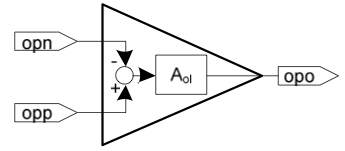
\includegraphics[height=2cm, valign=t]{./pictures/opAmpOL.png}
	\end{center}
		& \vspace{-7mm}
          \begin{center}
			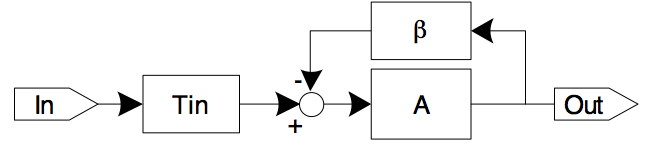
\includegraphics[height=2cm, valign=t]{./pictures/opAmpCL.png}
		  \end{center}\\
	\hline
	\multicolumn{2}{|c|}{\textbf{Frequenzgänge}}\\
	\hline
	\large{$A_{ol}(s)=\frac{A_{ol_0}}{(1+\frac{s}{\omega_{p_{ol_1}}})(1+\frac{s}{\omega_{p_{ol_2}}})\dots}$}
	& $\begin{aligned}
        A_{cl}(s) &= \frac{A_{cl_0}}{(1+\frac{s}{\omega_{p_{cl_1}}})(1+\frac{s}{\omega_{p_{cl_2}}})\dots} = \frac{T_{in}(s)\cdot A_{ol}(s)}{1+\beta(s)\cdot A_{ol}(s)}\\
		\beta(s) &= \frac{V_{opn}}{V_{out}}\;\text{oder}\;\frac{V_{opp}}{V_{out}}\\
		T_{in}(s) &= \frac{V_{opn}}{V_{in}}\;\text{oder}\;\frac{V_{opp}}{V_{in}}\\
        V_{out} &= A_{cl}(s)\cdot V_{in} = \frac{T_{in}(s)\cdot A_{ol}(s)}{1 + \underbrace{A_{ol}(s)\cdot \beta(s)}_{T_s(s):Loop-Gain}} \cdot V_{in}
	   \end{aligned}$\\
	\hline
\end{tabular}
\\ \\
\begin{tabular}{m{0.45\linewidth}m{0.45\linewidth}}
	Durch das Schliessen des Loops wird die Bandbreite vergrössert, das gain-bandwidth-product(GBP) bleibt jedoch konstant. Die Verstärkung wird jedoch um $T_{s0}(s)$ (Linearer Loop Gain) reduziert. Der Phasengang wird durch das Verschieben des ersten Poles auch verändert, wie folgende Grafik zeigt.
	& \begin{center}
        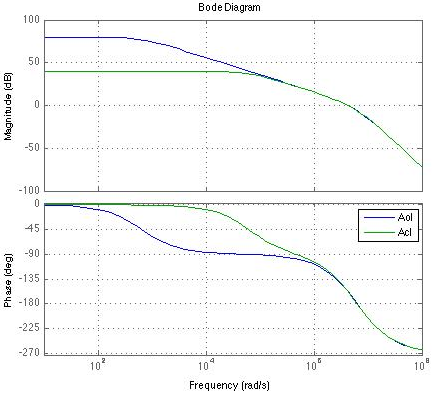
\includegraphics[width=6.7cm, valign=t]{./pictures/AolAcl.png}
    \end{center}
\end{tabular}
\vspace{-7mm}
\subsection{Stabilität des Systems}
\begin{tabular}{m{0.45\linewidth}m{0.45\linewidth}}
    Um die Stabilität des OpAmps zu betrachten, wird der Loop geöffnet. Damit das System stabil ist, darf das       
    Fehlersignal sich selbst nicht verstärken. Damit dies der Fall ist muss die Phase $>-180^\circ$ sein bei einem Loop Gain von $1$, da das Vergleichsglied die Phase noch um $180^\circ$ dreht. 
    
    Ein Mass für die Stabilität ist die 
    Phasenmarge (Phase Margin) und die Verstärkungsmarge (Gain Margin). Optimal ist ein Phase Margin von $60^{\circ}$.
    
    Die UTF ist dann stabil, wenn sie nie $\infty$ wird d.h der Nenner darf nie 0 werden.
    & \begin{center}
        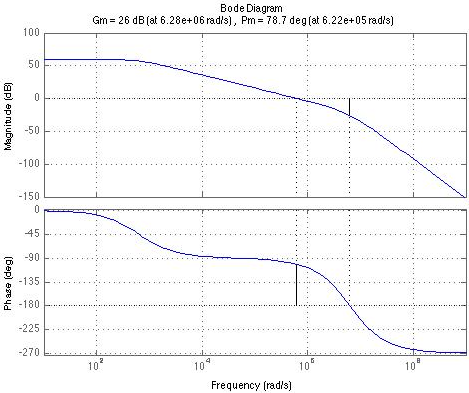
\includegraphics[width=5cm, valign=t]{./pictures/margins.png}
    \end{center}
\end{tabular}

% ----------------------------------------------------------------------------------------------------  
\subsection{OP als Regelkreis}  
\vspace{-1.5\topsep}
\begin{longtable}[t]{|p{5cm}|p{12.7cm}|}
    \hline  
    \multicolumn{2}{|l|}{\bf Nicht-invertierender OP}
    \\ \hdashline
    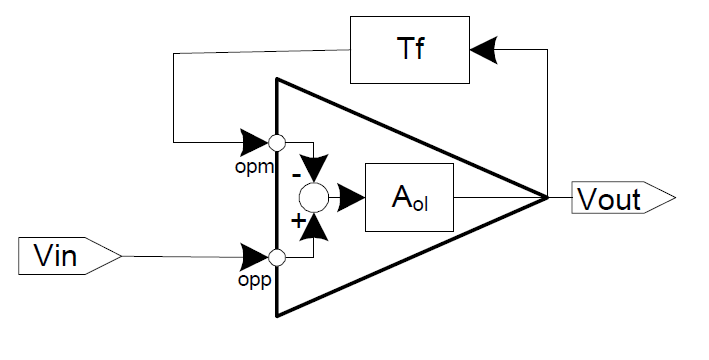
\includegraphics[width=5cm, valign=t]{pictures/opAmpNI.png}\newline\newline
    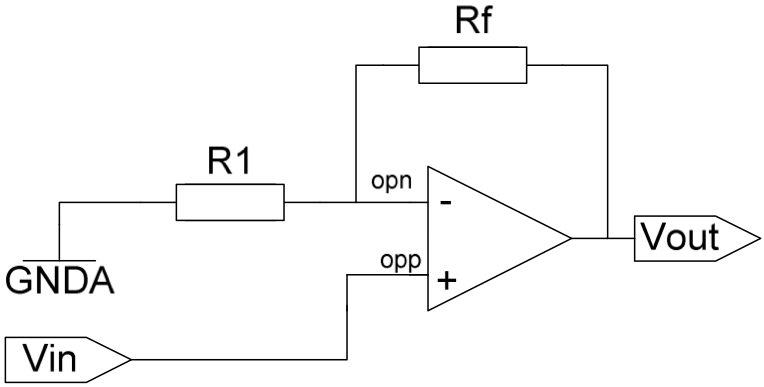
\includegraphics[width=5cm]{pictures/OPnichtInv.png}
    & {\vspace{-1.5\topsep}
        \begin{align*}
            A &= A_{ol}\\
            T_{in} &= 1\\
            \beta &= T_f = \frac{R_1}{R_1 + R_f} = \frac{1}{T}\\
            \frac{V_{out}}{V_{in}} &= \textcolor{red}{T = \frac{T_{in}}{\beta}\cdot \frac{1}{1+ \frac{1}{\beta 
            \cdot A_{ol}}} = \frac{T_{in}\cdot A_{ol}}{1 + A_{ol}\cdot \beta}} = 
            \frac{A_{ol}}{1 + A_{ol} \cdot \frac{R_1}{R_1 + R_f}} \approx \frac{R_1 + R_f}{R_1} =\frac{1}{\beta}
        \end{align*}
    }
    \\ \hline
% ---------------------------------------------------------------------------------------------------- 
    \multicolumn{2}{|l|}{\bf Invertierender OP}
    \\ \hdashline
    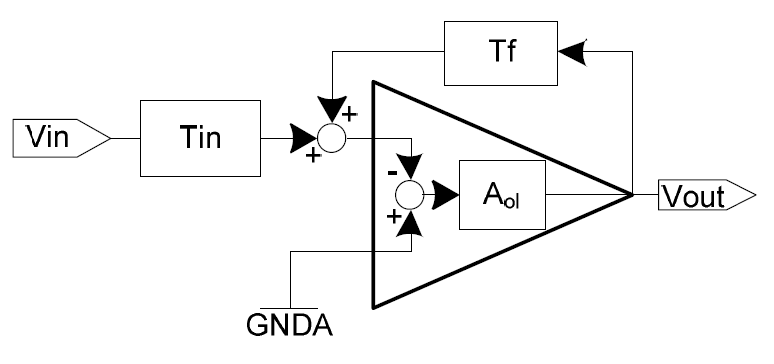
\includegraphics[width=5cm, valign=t]{pictures/opAmpInv.png}\newline\newline
    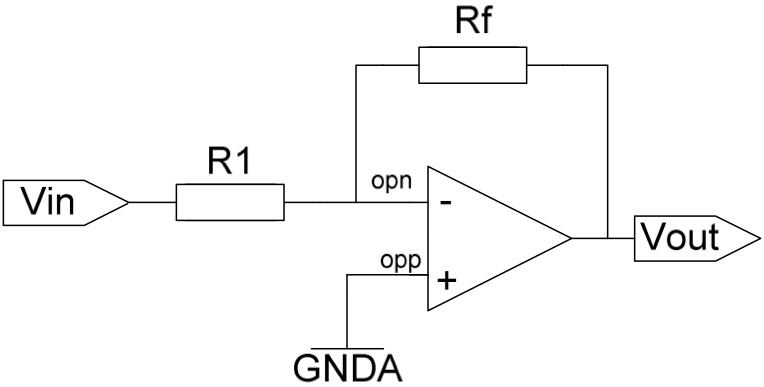
\includegraphics[width=5cm]{pictures/OPInv.png}
    & {\vspace{-1.5\topsep}
        \begin{align*}
            A &= A_{ol}\\
            T_{in} &= \frac{R_f}{R_1 + R_f} = 1 - \beta\\
            \beta &= T_f = \frac{R_1}{R_1 + R_f} = \frac{1}{1-T}\\
            \frac{V_{out}}{V_{in}} &= \textcolor{red}{T = -\frac{T_{in}}{\beta}\cdot 
            \frac{1}{1+ \frac{1}{\beta \cdot A_{ol}}}} =
            \frac{-T_{in} \cdot A_{ol}}{1+A_{ol} \cdot \beta}\approx -\frac{R_f}{R_1} = -\frac{1-\beta}{\beta}
        \end{align*}
    }
    \\ \hline
\end{longtable}
% ---------------------------------------------------------------------------------------------------- 
\vspace{-2.5\topsep}
\begin{longtable}[t]{|p{5cm}|p{12.7cm}|}
    \hline  
    \multicolumn{2}{|l|}{\bf Closed-Loop-Frequenzgang}
    \\ \hdashline
    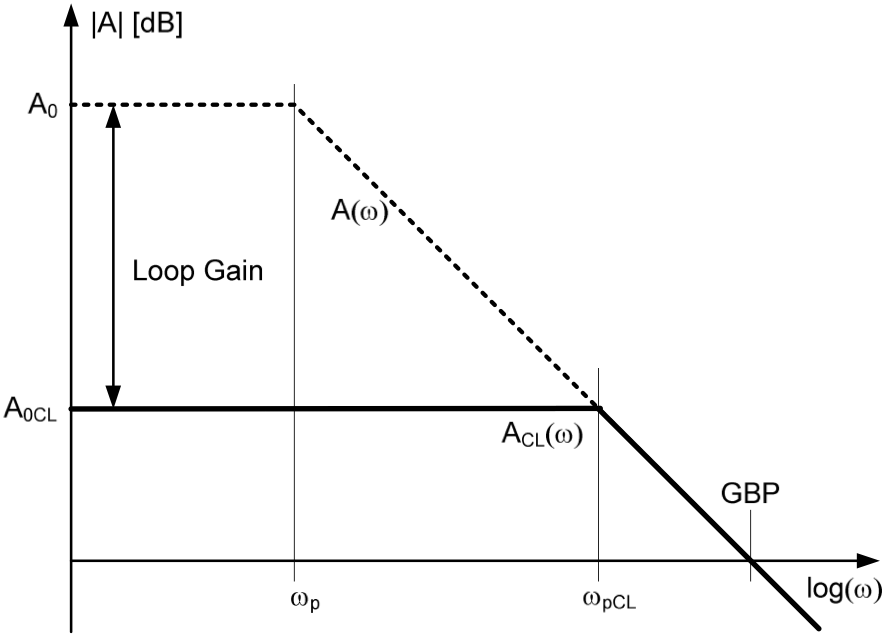
\includegraphics[width=5cm, valign=t]{pictures/ClosedLoopFreqGang.png}
    & {\vspace{-1.5\topsep}
        \begin{align*}
            \intertext{Frequenzabhängige Verstärkung Opamp:}
            A_{ol}(s) &= \frac{A_0}{1 + s/\omega_p} = \frac{A_0}{1+\frac{A_0}{2\pi \cdot GBP} \cdot s}\\
            \intertext{eingesetzt in folgende Formel:}
            V_{out} &= \frac{A_{ol}}{1 + \beta \cdot A_{ol}} \cdot V_{in}\\
            \intertext{ergibt:}
            A_{cl}(s) &= \frac{\frac{A_0}{1 + s/\omega_p}}{1 + \beta \frac{A_0}{1 + s/\omega_p}} = 
            \frac{A_0}{(1 + A_0 \beta) + s/\omega_p} = 
            \frac{\textcolor{red}{\frac{A_0}{1 + A_0 \beta}}}{1 + s \frac{1}
            {\textcolor{blue}{\omega_p(1 + A_0 \beta)}}} = 
            \frac{\textcolor{red}{A_{0_{cl}}}}{1 + s\frac{1}{\textcolor{blue}{\omega_{p_{cl}}}}}
        \end{align*}
        \newline
        Für $\mathrm{A_0 \cdot \beta \gg 1}$ gilt:\newline
        \vspace{-1.5\topsep}
        \begin{itemize}[leftmargin=*]
            \item Verstärkung $\mathrm{A_{0cl} = 1/\beta}$
            \item Bandbreite wird vergrössert um den Faktor $\mathrm{A_0 \cdot\beta}$
            \newline
        \end{itemize}
        \begin{tabular}{lp{8cm}}
          $\left.\begin{matrix}
            \mathrm{GBW = A_0 \cdot \omega_p}\\
            \mathrm{GBP = \dfrac{A_0 \cdot \omega_p}{2\pi}}
          \end{matrix}\right\rbrace$ &
          Frequenz bei welcher der Amplitudengang der Verlängerung des 1.Pols die 0dB-Linie schneidet.
        \end{tabular} \newline
        Closed-Loop-Bandbreite: Schnittpunkt $\mathrm{A_{cl}}$ mit $\mathrm{A(\omega)}$\newline
        Loop Gain: $A_{ol}(s) \cdot \beta = A(s) \cdot \beta$ oder $A_{0_{dB}} - A_{0cl_{dB}}$ (nach Grafik) \newline
        Unity-Gain: Frequenz wo der Amplitudengang (aller Pole) die 0dB-Linie schneidet.
    }
    \\ \hline
\end{longtable}


\subsection{DC-Betrachtung: (endliche Verstärkung $\mathrm{A_{ol}}$)}
\begin{itemize}
    \item Eingangsdifferenzspannung: $\mathrm{\frac{V_{out}}{A_{ol}}}$
    \item Verstärkungsfehler: $\mathrm{\sim\frac{1}{\beta \cdot A_{ol}}}$
    \item Eingangsimpedanz vergrössert um $\mathrm{\beta \cdot A_{ol}}$
    \item Ausgangsimpedanz dividiert durch $\mathrm{\beta \cdot A_{ol}}$
  \end{itemize}  
